\documentclass[10pt]{article}

\pagestyle{empty}

\setlength{\textheight}{250mm}
\setlength{\textwidth}{180mm}
\setlength{\oddsidemargin}{-8mm}
\setlength{\topmargin}{-1.5cm}

\usepackage{amsmath}
\usepackage{amsthm}
\usepackage{psfrag}
\usepackage{graphicx}
\usepackage{bm}
\usepackage{mathrsfs}
\usepackage{icomma} % pacchetto per limitare lo spazio standard posto dopo la virgola in caso che la virgola sia tra cifre
\usepackage{amsfonts} % amplia i caratteri matematici disponibili
\usepackage{amssymb}
%\usepackage{wrapfig}
\usepackage{empheq}

\usepackage{epstopdf}
\usepackage[utf8x]{inputenc}
\usepackage{ifthen}
\usepackage{subfig}

\usepackage[italian]{babel}
%\usepackage[latin1]{inputenc}

\usepackage{pgfplots}
\pgfplotsset{compat=1.9}

%\input{def}

%\newcommand{\kg}{\textrm{kg}}
%\newcommand{\K}{\textrm{K}}
%\newcommand{\m} {\textrm{m}}
%\newcommand{\dm}{\textrm{dm}}
%\newcommand{\cm}{\textrm{cm}}
%\newcommand{\mm}{\textrm{mm}}
%\newcommand{\s} {\textrm{s}}
%\newcommand{\N} {\textrm{N}}
%\renewcommand{\Pa}{\textrm{Pa}}

\def \flagSect{0} % 1    : numerazione
		  % else : niente
%\newcommand{\taitol}[1]  % stile titolo
%{
%%{\textit{#1}}
%{#1}
%}
\def \soluzione{Soluzione}
\def \partePrima{Concetti. }
\def \parteSeconda{Svolgimento. }
%\def \parteTerza{}
\newcommand{\sol}{\subsubsection*{\soluzione}}
\newcommand{\partone}{\ \ \ \ \ \textbf{\partePrima}}
\newcommand{\parttwo}{\vspace{0.2cm}\textbf{\parteSeconda}}

\ifnum\flagSect=1
\newtheorem{esercizio}{Esercizio}%[section]
\else
\newtheorem*{esercizio}{Esercizio}
\fi

\newtheorem*{teorema}{Teorema}
\newtheorem*{lemma}{Lemma}

% ###########################################################
%\def \flagSect{0} % 1    : numerazione
		  % else : niente
%\newcommand{\taitol}[1]  % stile titolo
%{
%%{\textit{#1}}
%{#1}
%}
\def \soluzione{Soluzione}
\def \partePrima{Concetti. }
\def \parteSeconda{Svolgimento. }
%\def \parteTerza{}
\newcommand{\sol}{\subsubsection*{\soluzione}}
\newcommand{\partone}{\ \ \ \ \ \textbf{\partePrima}}
\newcommand{\parttwo}{\vspace{0.2cm}\textbf{\parteSeconda}}

\ifnum\flagSect=1
\newtheorem{esercizio}{Esercizio}%[section]
\else
\newtheorem*{esercizio}{Esercizio}
\fi

\newtheorem*{teorema}{Teorema}
\newtheorem*{lemma}{Lemma}

% ###########################################################
%\def \flagSect{0} % 1    : numerazione
		  % else : niente
%\newcommand{\taitol}[1]  % stile titolo
%{
%%{\textit{#1}}
%{#1}
%}
\def \soluzione{Soluzione}
\def \partePrima{Concetti. }
\def \parteSeconda{Svolgimento. }
%\def \parteTerza{}
\newcommand{\sol}{\subsubsection*{\soluzione}}
\newcommand{\partone}{\ \ \ \ \ \textbf{\partePrima}}
\newcommand{\parttwo}{\vspace{0.2cm}\textbf{\parteSeconda}}

\ifnum\flagSect=1
\newtheorem{esercizio}{Esercizio}%[section]
\else
\newtheorem*{esercizio}{Esercizio}
\fi

\newtheorem*{teorema}{Teorema}
\newtheorem*{lemma}{Lemma}

% ###########################################################
%\input{logicNumb}
%\newcommand{\sectionIf}[2]
%{
%   \ifthenelse{\equal{#1}{1}}
%              {\subsection{#2}}{\subsection*{#2}}
%}
% ###########################################################

%\newcommand{\sectionIf}[2]
%{
%   \ifthenelse{\equal{#1}{1}}
%              {\subsection{#2}}{\subsection*{#2}}
%}
% ###########################################################

%\newcommand{\sectionIf}[2]
%{
%   \ifthenelse{\equal{#1}{1}}
%              {\subsection{#2}}{\subsection*{#2}}
%}
% ###########################################################



\begin{document}

\begin{center}
\textbf{Esercizi per il corso di Fluidodinamica} 
\medskip
\end{center}


\begin{minipage}[l]{0.55\textwidth}
 \begin{exerciseS}[Getto piano turbolento]
  Calcolare la soluzione in similitudine per un getto turbolento piano.

 \end{exerciseS}

\partone
 Equazioni mediate di Reynolds. Equazioni di Prandtl per lo strato
 limite turbolento. Correnti debolmente non parallele. Soluzioni in
 similitudine. Entrainment.
%\begin{itemize}
%      
%\end{itemize}

\end{minipage}
\hspace{3mm}
\begin{minipage}[r]{0.45\textwidth}
  \centering
  \vspace{5mm}
  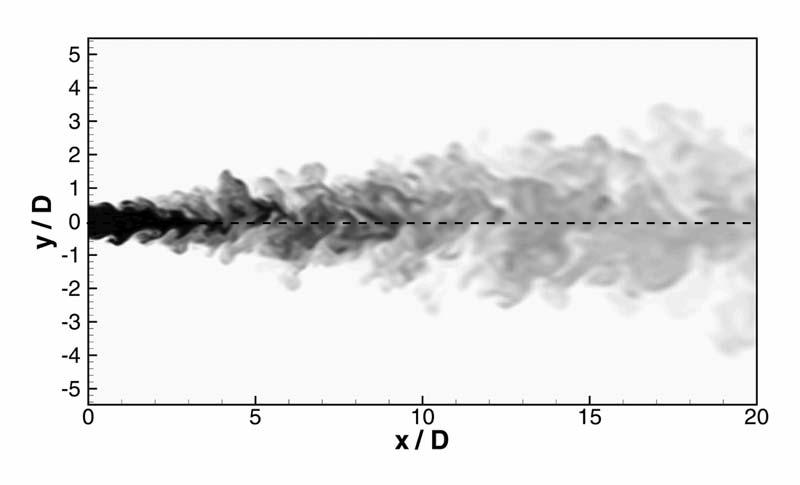
\includegraphics[width=1.0\textwidth]{./fig/turbulentJet}
\end{minipage}

% ---------------------------------------------------------------------------

\sol
Si descrive schematicamente il procedimento:
\begin{itemize}
\item Il problema turbolento viene descritto dalle equazioni mediate di Reynolds.
\item I problemi di "strato limite" possono essere ben descritti dalle equazioni
      di Prandtl, ricavabili grazie a ragionamenti sugli ordini di grandezza,
      analoghe alle equazioni di Prantdl laminari.
\item Viene introdotta una variabile di similitudine $\eta$; si ipotizza
      la forma della soluzione: $u = U_0 f$, $\langle u'v' \rangle = U_0^2 g$
\item Vengono calcolati i flussi integrali di massa, quantità di moto ed energia
      cinetica.
\item Si inserisce l'ansatz sulla soluzione nelle equazioni di Prandtl per
      ottenere un'equazione per i profili similari di velocità $f$ e degli 
      sforzi turbolenti $g$.
      Si ricava l'andamento dello spessore dello $\delta(x)$``strato limite'',
      necessario affinché esista una soluzione similare.
\item Per ottenere una equazione chiusa, si introduce l'ipotesi di Boussinesq, che
      lega $f$ e $g$. Infine si risolve, con le opportune condizioni al contorno,
      l'equazione in $f$.

\end{itemize}


\parttwo
\begin{itemize}
\item Il punto di partenza del problema sono le equazioni mediate di
 Reynolds (RANS)
 \begin{equation}
  \begin{cases}
   (\bm{U} \cdot \bm{\nabla}) \bm{U}
  + \bm{\nabla} \cdot \langle \bm{u}' \otimes \bm{u}'  \rangle
  - \dfrac{1}{Re} \nabla^2 \bm{U} + \bm{\nabla} P = 0   \\
   \bm{\nabla} \cdot \bm{U} = 0
  \end{cases}
 \end{equation}
 ottenibili inserendo la decomposizione di Reynolds delle variabili in
 moto medio e fluttuazione $\bm{u} = \bm{U} + \bm{u}'$ all'interno delle
 equazioni di Navier-Stokes.

 Se si considera un problema bidimensionale (per le grandezze medie),
  le RANS in coordinate cartesiane sono
 \begin{equation}
 \begin{cases}
U \dfrac{\partial U}{\partial x} + V \dfrac{\partial U}{\partial y} 
+ \dfrac{\partial \langle u'u' \rangle}{\partial x}  
+ \dfrac{\partial \langle u'v' \rangle}{\partial y}  
- \dfrac{1}{Re} \left( \dfrac{\partial^2 U }{\partial x^2} 
                    +  \dfrac{\partial^2 U }{\partial y^2} \right)
+\dfrac{\partial P}{\partial x} = 0 \\
U \dfrac{\partial V}{\partial x} + V \dfrac{\partial V}{\partial y} 
+ \dfrac{\partial \langle u'v' \rangle}{\partial x}  
+ \dfrac{\partial \langle v'v' \rangle}{\partial y}  
- \dfrac{1}{Re} \left( \dfrac{\partial^2 V }{\partial x^2} 
                    +  \dfrac{\partial^2 V }{\partial y^2} \right)
+\dfrac{\partial P}{\partial y} = 0 \\
\dfrac{\partial U}{\partial x} + \dfrac{\partial V}{\partial y} = 0 
 \end{cases}
 \end{equation}

\item Per problemi ``di strato limite'' le equazioni RANS possono essere
 semplificate, considerando gli ordini di grandezza delle coordinate e 
 dei campi che compaiono all'interno delle equazioni.
 Per la regione ``interna'' (la lunghezza caratteristica in y è ``molto 
 minore'' di quella in x), assumendo che la pressione ``esterna'' sia
 costante e trascurando i termini di fluttuazione con contributo minore 
 \begin{equation}
 \begin{cases}
U \dfrac{\partial U}{\partial x} + V \dfrac{\partial U}{\partial y} 
+ \dfrac{\partial \langle u'v' \rangle}{\partial y}  
- \dfrac{1}{Re} \dfrac{\partial^2 U }{\partial y^2}
+\dfrac{\partial P}{\partial x} = 0 \\
 \dfrac{\partial \langle v'^2 \rangle}{\partial y}  
+\dfrac{\partial P}{\partial y} = 0 \\
\dfrac{\partial U}{\partial x} + \dfrac{\partial V}{\partial y} = 0 
 \end{cases}
 \end{equation}
 Da queste prime semplificazioni, a differenza delle equazioni di 
 strato limite per il caso laminare, la pressione non è funzione solo
 della coordinata $x$, ma $P+\langle v'^2 \rangle$ è funzione solo di
 $x$. Con ulteriori considerazioni sui termini di fluttuazione nel caso
 di getti, è possibile scrivere in prima approssimazione
 \begin{equation}
 \begin{cases}
U \dfrac{\partial U}{\partial x} + V \dfrac{\partial U}{\partial y} 
+ \dfrac{\partial \langle u'v' \rangle}{\partial y}  
- \dfrac{1}{Re} \dfrac{\partial^2 U }{\partial y^2} = 0 \\
P + \langle v'^2  \rangle = P_0(x) \\ 
\dfrac{\partial U}{\partial x} + \dfrac{\partial V}{\partial y} = 0 
 \end{cases}
 \end{equation}
 avendo indicato con $P_0(x)$ la pressione del problema esterno e avendo usato l'approssimazione $\partial P/\partial x = \partial P_0 / \partial x - \partial \langle v'^2 / \partial x \rangle \simeq \partial P_0 / \partial x = 0$. Le fluttuazioni
 nel problema esterno sono considerate nulle.

 Prima di procedere con la ricerca di soluzioni in similitudine, viene
 fatta l'ultima ipotesi: consideriamo numeri di Reynolds sufficientemente
 alti da rendere trascurabile l'effetto degli sforzi viscosi del moto
 medio rispetto agli effetti delle fluttuazioni.
 \begin{equation}
 \begin{cases}
U \dfrac{\partial U}{\partial x} + V \dfrac{\partial U}{\partial y} 
+ \dfrac{\partial \langle u'v' \rangle}{\partial y} = 0 \\ 
P + \langle v'^2  \rangle = P_0(x) \\ 
\dfrac{\partial U}{\partial x} + \dfrac{\partial V}{\partial y} = 0 
 \end{cases}
 \end{equation}


\item Partendo dalle equazioni di Prandtl turbolente semplificate, si
 introduce la variabile di similitudine
\begin{equation}
  \eta = \dfrac{y}{\delta(x)}
\end{equation}
 con $\delta(x)$ una grandezza caratteristica (convenzionale) della 
 sezione del getto; 
 si  ipotizzano poi il profilo di velocità della componente $x$ della
 velocità e del termine di fluttuazione $\langle u'v' \rangle$:
\begin{equation}
\begin{aligned}
 U(x,y) & = U_0 f(\eta(x,y)) \\
 \langle u'v' \rangle (x,y) & = U^2_0 g(\eta(x,y))
\end{aligned}
\end{equation}

 Si calcola la derivata parziale di U in x, che verrà usata in seguito:
\begin{equation}
\begin{aligned}
 \dfrac{\partial U}{\partial x} & =  U'_0 (x) f(\eta)
 - U_0(x) \frac{y \delta'(x)}{\delta^2(x)} f'(\eta) = \\
 & =  U'_0 (x) f(\eta)
 - U_0(x) \frac{ \delta'(x) \eta}{\delta(x)} f'(\eta)
\end{aligned}
\end{equation}

Tramite il vincolo di incomprimibilità si ricava la forma della 
 componente $V$ della velocità. Nel trasformare l'integrale su $y$
 in un integrale su $\eta$, si usa $y = \delta(x) \eta$,
 $d\xi = \delta(x) d\chi$.
\begin{equation}
\begin{aligned}
 V(x,y) - \underbrace{V(x,0) }_{=0} & =
 \int_{\xi=0}^y \dfrac{\partial V(x,\xi)}{\partial y} d\xi = 
 -\int_{\xi=0}^y \dfrac{\partial U(x,\xi)}{\partial x}  = \\
 & = -\int_{\chi=0}^\eta \left[ U'_0 (x) f(\chi)
 - U_0(x) \frac{ \delta'(x) \chi}{\delta(x)} f'(\chi) \right]
  \delta(x) d \chi = \\
 & = -\int_{\chi=0}^\eta \left[ \delta(x) U'_0 (x) f(\chi)
 - U_0(x) \delta'(x) \chi f'(\chi) \right]
   d \chi
\end{aligned}
\end{equation}

\item Prima di scrivere le equazioni di Prandtl per le variabili
 adimensionali, conviene calcolare il flusso di quantità di moto
 in direzione $x$ attraverso dei piani verticali. Questo consente
 di trovare una relazione tra $U_0$ e $\delta$ da usare in seguito.
 \begin{equation}
  Q = \rho \int_{y=-\infty}^\infty U^2(x,y) dy
 \end{equation}
 Si calcola la derivata in direzione $x$ di $Q$, usando le equazione
 di Prandtl della componente $x$ della quantità di moto:
\begin{equation}
 \dfrac{d Q}{d x}=\dfrac{d}{d x}\rho \int_{y=-\infty}^\infty U^2(x,y) dy = 
  \rho \int_{y=-\infty}^\infty \dfrac{\partial U^2}{\partial x} dy =
  -\rho \int_{y=-\infty}^\infty \dfrac{\partial UV}{\partial y} 
  + \dfrac{\partial \langle u'v' \rangle}{\partial y} dy = 0
\end{equation}
 se si considera un fluido in quiete all'infinito.
 Utilizzando i profili in similitudine
\begin{equation}
\begin{aligned}
 0 = \dfrac{d Q}{d x} & = 
  \dfrac{d}{dx} \int_{y=-\infty}^\infty  U^2 dy = \\ 
& = \dfrac{d}{dx} \left( U^2_0(x) \delta(x) \right)
   \int_{\eta=-\infty}^{\infty} f^2(\eta)d\eta
\end{aligned}
\end{equation}
Deve quindi essere $ \frac{d}{dx}(U_0^2 \delta)= 0$, cioè
\begin{equation}
 2 U_0 U'_0 \delta + U^2_0 \delta' = 0 \qquad \Rightarrow \qquad
 \delta\dfrac{U'_0}{U_0} = -\dfrac{1}{2}\delta'
\end{equation}

\item Inseriamo ora la forma di $U$, $V$, $\langle u'v' \rangle$ 
 espresse in termini della variabile e delle funzioni di similitudine
 nella componente $x$ dell'equazione della quantità di moto.

\begin{equation}
 U_0 f \left[ U'_0 f - U_0 \dfrac{\delta'}{\delta} \eta f' \right]
 - \left[ \int_{\chi=0}^\eta \left[ \delta(x) U'_0 (x) f(\chi)
 - U_0(x) \delta'(x) \chi f'(\chi) \right]d \chi \right]
 \dfrac{U_0}{\delta} f' + \dfrac{U_0^2}{\delta} g' = 0
\end{equation}
Moltiplicando per $\dfrac{\delta}{U_0^2}$ e integrando per parti
 l'integrale che contiene $\eta f'(\eta)$
\begin{equation}
 \delta\dfrac{U'_0}{U_0} f^2 - \delta' \eta f f' 
- \delta\dfrac{U'_0}{U_0} f' \int_0^\eta f d \chi
+ \delta' f'(\eta) \left[ \chi f(\chi) \right]\bigg|_0^\eta
- \delta'  f(\eta)\int_0^\eta f(\chi)d\chi + g'(\eta) = 0
\label{eq:sim}
\end{equation}
 Usando la relazione tra $U_0$  e $\delta$ trovata al punto precedente
 è possibile scrivere l'equazione come
\begin{equation}
 \dfrac{1}{2} \delta'(x) \left[ f^2(\eta)
 + f'(\eta)\int_{\chi=0}^{\eta} f(\chi) d\chi  \right] = g'(\eta) 
\end{equation}
Affinchè sia possibile trovare una soluzione in similitudine, non ci
 possono essere coefficienti dipendenti da $x$ o $y$ se non tramite
 $\eta$. Deve quindi essere:
\begin{equation}
 \delta'(x) = S \qquad \Rightarrow \qquad \delta(x) = S (x-x_0)
\end{equation}
Seguendo questo procedimento è stato possibile ottenere una stima 
 dell'evoluzione in $x$ della grandezza trasversale caratteristica
 $\delta(x)$: la grandezza trasversale caratteristica di un getto
 turbolento è lineare in $x$. Dalla costanza del flusso di 
 quantità di moto $U_0^2(x)\delta(x) = \text{cost}$ e quindi la 
 velocità caratteristica del getto evolve come
 \begin{equation}
  U_0(x) \sim x^{-1/2}
 \end{equation}

\item Come fatto in precedenza per il flusso di quantità di moto
 (costante in $x$), vengono calcolate le derivate in $x$ dei flussi
 di massa e di energia cinetica del moto medio per la soluzione in
 similitudine attraverso piani perpendicolari all'asse $x$.
 Il flusso di massa $M$ è:
 \begin{equation}
 \begin{aligned}
   M & = \rho \int_{y=-\infty}^{\infty} U dy =
     \rho U_0(x)\delta(x) \int_{\eta=-\infty}^{\infty} f(\eta) d \eta \sim
     x^{1/2}   \\ \\
   \frac{d M}{dx} & \sim x^{-1/2} > 0  , \ \ \text{per $x>0$}
 \end{aligned}
 \end{equation}
 Il flusso di massa aumenta allontanandosi dall'ugello. Il getto
 riesce a ``trascinare'' anche del fluido che non esce dall'ugello
 (entrainment). Il flusso di energia cinetica del moto medio è:
 \begin{equation}
 \begin{aligned}
   E & = \dfrac{1}{2} \rho \int_{y=-\infty}^{\infty} U^3 dy =
    \dfrac{1}{2} \rho U_0^3(x)\delta(x) 
    \int_{\eta=-\infty}^{\infty} f^3(\eta) d\eta \sim x^{-1/2} \\ \\
   \frac{d E}{dx} & \sim -x^{-3/2} < 0, \ \ \text{per $x>0$} 
 \end{aligned}
 \end{equation}
 Il flusso di energia cinetica del moto medio diminuisce allontanandosi
 dall'ugello, nonostante l'equazioni utilizzate nella soluzione in
 similitudine non contengano il termine dissipativo degli sforzi viscosi,
 che quindi non può avere nessuna influenza sulla diminuzione 
 di energia cinetica del moto medio: l'energia del moto medio viene
 trasferita alle fluttuazioni di velocità. Scrivendo le equazioni
 di bilancio dell'energia cinetica del moto medio e dell'energia cinetica
 delle fluttuazioni (energia turbolenta) si trovano due termini opposti:
 il termine che in generale fa diminuire l'energia cinetica del moto
 medio, si trova nell'equazione dell'energia turbolenta con segno
 opposto.

\item Nell'eq.~\ref{eq:sim}, anche dopo aver sostituito $\delta' = S$, 
 rimangono due equazioni incognite $f(\eta)$, $g(\eta)$. Così come 
 le RANS non sono un problema chiuso, anche il problema semplificato
 non è chiuso.
 Per ottenere una soluzione si può introdurre l'ipotesi di Boussinesq
 (validità di questa ipotesi? Nessuna giustificazione rigorosa \dots)
 per esprimere il termine di fluttuazioni in funzione del moto medio.
 Per il getto piano, l'ipotesi di Boussinesq si riduce a
 \begin{equation}
  - \langle u'v' \rangle = \nu_T \dfrac{\partial U}{\partial y}
 \end{equation}
 avendo indicato con $\nu_T$ la viscosità turbolenta.
 \begin{gather}
  - U^2_0 g(\eta) = \nu_T \dfrac{U_0}{\delta(x)} f(\eta) \\
   g(\eta) = - \dfrac{\nu_T}{U_0(x)\delta(x)} f(\eta) \\
 \end{gather}
 Fatte già molte ipotesi (non tutte con fondamento fisico), facciamo 
 l'ultima ipotesi che consente di ottenere una soluzione in forma 
 chiusa del problema. Si ipotizza che 
 \begin{equation}
  \hat{\nu}_T = \dfrac{\nu_T}{U_0(x)\delta(x)} = \text{cost}
  \qquad \Rightarrow \qquad g(\eta) = - \nu_T f'(\eta)
 \end{equation}

% \begin{center}
 \textbf{La validità di queste ipotesi andrà controllata
 a posteriori.}
% \end{center}

 L'equazione in $f(\eta)$ diventa:
 \begin{equation}
  \dfrac{1}{2} S \left[ f^2(\eta)
    + f'(\eta)\int_{\chi=0}^{\eta} f(\chi) d\chi \right] = 
    - \hat{\nu}_T f'''(\eta)
 \end{equation}
 Si introduce la funzione $F(\eta) = \int_{\chi=0}^{\eta} f(\chi)d\chi$
 per eliminare il termine integrale e ottenere un'equazione differenziale
 in $F(\eta)$ (osservare che $F'(\eta) = f(\eta)$ e $F(0)=0$ poiché
 l'intervallo di integrazione ha dimensione nulla):
 \begin{gather}
   \dfrac{1}{2}S \left( F'^2 + F'' F \right) = -\hat{\nu}_T F''' \\
   \dfrac{1}{2}S \left( F'F \right)' = -\hat{\nu}_T F''' \\
 \end{gather}
 Le condizioni di simmetria sull'asse del getto sono
 \begin{equation}
  \begin{aligned}
   \frac{\partial U}{\partial y}(x,y=0) = 0 \quad \Rightarrow \quad
     f'(\eta=0) = 0 \quad \Rightarrow \quad F''(\eta=0) = 0
  \end{aligned}
 \end{equation}

 Si integra ora due volte. Dopo aver integrato la prima volta, la prima
 costante di integrazione è nulla dalle condizioni $F(0)=0$, $F''(0)=0$.
 Si integra la seconda volta e si definisce la velocità di riferimento
 $U_0(x)$ (fino ad ora generica) con la condizione $F'(0) = f(0) = 1$:
 ricordando $U(x,y) = U_0(x) f(\eta(x,y))$, si ottiene che $U_0(x)$ è
 la velocità sull'asse ($y=0$, $\eta=0$).
 
 \begin{equation}
 \begin{aligned}
 & \frac{1}{2}S\ F'(\eta)F(\eta) + \hat{\nu}_T F''(\eta) = C 
    \stackrel{\text{b.c}}{=}0  & ( (F^2)' = 2FF') \\
 & \dfrac{1}{4} S (F^2)' + \hat{\nu}_T F'' = 0 & ( integrare ...)  \\
 & F' = -\dfrac{S}{4\hat{\nu}_T} F^2 + B \stackrel{F'(0)=1}{=} 
  1 - \dfrac{S}{4\hat{\nu}_T} F^2 & 
 \end{aligned}
 \end{equation}

 Integrando un'ultima volta si ottiene la soluzione $F(\eta)$, la cui 
 derivata $f(\eta)$ è il profilo in similitudine della velocità $U$
 \begin{equation}
  F(\eta) = \dfrac{1}{\alpha}\tanh{(\alpha \eta)} \quad \Rightarrow \quad
  f(\eta) = \dfrac{1}{\cosh^2{(\alpha \eta)}} = \dfrac{U(x,y)}{U_0(x)}
 \end{equation}
 con $\alpha = \sqrt{\dfrac{S}{4\hat{\nu}_T}}$.

 Mancano da determinare
 i valori delle costanti che compaiono nella soluzione, ottenibili usando
 dei confronti con le misure sperimentali e
 introducendo una definizione per la dimensione di riferimento $\delta(x)$ 
 della dimensione trasversale del getto: di solito si definisce 
 $\delta(x) = r_{1/2}(x)$ l'ordinata in cui la velocità $U(x,\delta(x))$
 è la meta
 della velocità sull'asse (o sul piano di simmetria), cioè
 \begin{equation}
   U(x,r_{1/2}(x)) = \dfrac{1}{2}U(x,0) = \dfrac{1}{2}U_0(x)
 \end{equation}
 Per questa scelta di $\delta(x)$ il coefficiente S risulta $S \sim 0.1$.
 

\begin{figure}
\begin{center}
\begin{tikzpicture}
  \begin{axis}[axis lines =center,
    disabledatascaling,
    anchor=origin,
    xlabel = $\eta$, ylabel =$f(\eta)$, 
    ymax=1.2, ymin=-0.2, xmax=5.2, xmin=-5.2,
    ytick={ 0, 0.2, ...,1.0}, xtick={-5, -4, ...,5}]
    \addplot
    [domain=-5.0:5.0,samples=50,smooth,thick,blue]
     {1/(cosh(x))^2};
  \end{axis}
\end{tikzpicture}
\end{center}
\caption*{Profilo di velocità similare $f(\eta)$ in variabile di
  similitudine $\eta$.}
\end{figure}



% \begin{center}
% \begin{tikzpicture}
% \draw[help lines, color=gray!30, dashed] (-4.9,-0.4) grid (4.9,1.4);
% \draw[->,ultra thick] (-5,0)--(5,0) node[below]{$x$};
% \draw[->,ultra thick] (0,-5)--(0,5) node[left]{$y$};
% \addplot
% [domain=-3.0:3.0,samples=40,smooth,thick,blue]
% {1/(cosh(x))^2};
% \end{tikzpicture}
% \end{center}

\end{itemize}

%%%%%%%%%%%%%%%%%%%%%%%%%%%%%%%%%%%%%%%%%%%%%%%%%%%%%%%%%%%%%%%%%%

%%%%%%%%%%%%%%%%%%%%%%%%%%%%%%%%%%%%%%%%%%%%%%%%%%%%%%%%%%%%%%%%%%

%%%%%%%%%%%%%%%%%%%%%%%%%%%%%%%%%%%%%%%%%%%%%%%%%%%%%%%%%%%%%%%%%%



%%%%%%%%%%%%%%%%%%%%%%%%%%%%%%%%%%%%%%%%%%%%%%%%%%%%%%%%%%%%%%%%%%

%%%%%%%%%%%%%%%%%%%%%%%%%%%%%%%%%%%%%%%%%%%%%%%%%%%%%%%%%%%%%%%%%%
%%%%%%%%%%%%%%%%%%%%%%%%%%%%%%%%%%%%%%%%%%%%%%%%%%%%%%%%%%%%%%%%%%

\end{document}
